\documentclass[fleqn, a4paper, 11pt, russian]{article}

\usepackage[utf8]{inputenc}
\usepackage[T1, T2A]{fontenc}
\usepackage[english, main = russian]{babel}
\usepackage{indentfirst}
\parindent 1.27cm
\usepackage{graphicx}
\usepackage{natbib}
\usepackage{caption, subcaption}
\usepackage[top=2cm, left=2cm, right=2cm, left=2cm]{geometry}
\usepackage{amsmath} %Для работы с матрицами
\usepackage{ragged2e}
\usepackage{makecell}

\graphicspath{{Images/}}

\captionsetup[figure]{name = Рисунок, labelsep = endash}
\captionsetup[table]{name = Таблица, labelsep = endash, justification=raggedright, singlelinecheck=false}
\setlength{\mathindent}{0pt}

\begin{document}
    \newcommand\tline[2]{$\underset{\text{#1}}{\text{\underline{\hspace{#2}}}}$}

\begin{titlepage}
	\centering
	{\fontsize{12pt}{5cm}\selectfont \bfseries Министерство образования и науки Российской Федерации} \\ \vspace{0.5cm}
	{\fontsize{7pt}{5cm}\selectfont ФЕДЕРАЛЬНОЕ ГОСУДАРСТВЕННОЕ АВТОНОМНОЕ ОБРАЗОВАТЕЛЬНОЕ УЧРЕЖДЕНИЕ ВЫСШЕГО ПРОФЕССИОНАЛЬНОГО ОБРАЗОВАНИЯ} \\ 
	\vspace{1cm}
	{\fontsize{12pt}{5cm}\selectfont \bfseries САНКТ-ПЕТЕРБУРГСКИЙ УНИВЕРСИТЕТ ИНФОРМАЦИОННЫХ ТЕХНОЛОГИЙ, МЕХАНИКИ И ОПТИКИ} \\ \vspace{1.5cm}

	{\fontsize{14pt}{5cm}\selectfont Кафедра \hspace{1cm} \underline{Систем Управления и Информатики}  \hspace{1cm} Группа \underline{Р3340}} \\ 
	\vspace{2cm}

	{\fontsize{20pt}{5cm}\selectfont \bfseries Лабораторная работа №7} \\
	{\fontsize{20pt}{5cm}\selectfont \bfseries “Анализ точности систем управления”} \\
	{\fontsize{14pt}{5cm}\selectfont Вариант - 2} \\
	\vspace{1.5cm}

	\flushleft

	{Выполнил \hspace{2cm} \underline{Алякин С.П.}\tline{(фамилия, и.о.)}{6.5cm} (подпись)} \\
	\vspace{2cm}

	{Проверил \hspace{2cm} \tline{(фамилия, и.о.)}{9cm} (подпись)} \\
	\vspace{5cm}

	"\underline{\hspace{0.7cm}}"\hspace{0.2cm}\underline{\hspace{2cm}}\hspace{0.2cm}20\underline{ 17 }г. \hspace{2cm} Санкт-Петербург, \hspace{2cm} 20\underline{ 17 }г. \\ \vspace{1cm}

	Работа выполнена с оценкой \hspace{1cm} \underline{\hspace{8cm}} \\ 
	\vspace{1cm}
	Дата защиты "\underline{\hspace{0.7cm}}"\hspace{0.2cm}\underline{\hspace{2cm}}\hspace{0.2cm}20\underline{ 17 }г.
		
\end{titlepage}
    \section*{Цель работы}
    Изучение математических моделей и исследование характеристик электромеханического объекта управления, построенного на основе электродвигателя постоянного тока независимого возбуждения.
    \section*{Исходные данные}
    \begin{table}[ht!]
    	\caption{Исходные данные}
    	\begin{tabular}{| c | c | c | c | c | c | c | c | c | c |}
    		\hline
    		\makecell{$U_\text{Н},$\\В} & \makecell{$n_0,$\\об/мин} & \makecell{$I_\text{Н},$\\A} & \makecell{$M_\text{Н},$\\Н$\cdot$м} & \makecell{R,\\Ом} & \makecell{$T_\text{Я},$\\мс} & \makecell{$J_\text{Д},$\\кг$\cdot$м$^2$} & \makecell{$T_\text{У},$\\мс} & $i_\text{Р}$ & \makecell{$J_\text{М},$\\кг$\cdot$м$^2$} \\
    		\hline
    		48 & 1000 & 12 & 5,5 & 0,75 & 5 & $1,6\cdot10^{-3}$ & 6 & 16 & 2,75\\
    		\hline
    	\end{tabular}
    \end{table}
    \clearpage
    \section{Расчёт параметров математической модели двигателя}
    Переведём заданное значение частоты в систему СИ
    \begin{align}
		n_0 = 1000 \text{ об/мин} = 104,72 \text{ рад/с} = \omega_0
    \end{align}
    Рассчитаем необходимые для создания модели параметры:
    \begin{align}
    	K_\text{У} &= \frac{U_\text{Н}}{U_m} = \frac{48}{10} &= 4,8\\
    	K_\text{Д} &= \frac{1}{R} = \frac{1}{0,75} &= 1,33\\
    	K_\text{М} &= \frac{M_\text{Н}}{I_\text{Н}} = \frac{5,5}{12} &= 0,4583\\
    	K_E &= \frac{U_\text{Н}}{\omega_0} = \frac{48}{104,72} &= 0,4583\\
    	J_\text{Р} &= 0,2J_\text{Д} = 0,2 \cdot 1,6\cdot10^{-3} &= 3,2\cdot10^{-4}\\
    	J_\Sigma &= J_\text{Д} + J_\text{Р} + \frac{J_\text{М}}{i_\text{Р}^2} = 1,6\cdot10^{-3} + 3,2\cdot10^{-4} + \frac{2,75}{16^2} &= 0,01266 \text{кг}\cdot\text{м}^2
	\end{align}
	\clearpage
	\section{Математическое моделирование электромеханического объекта}
	Составим математическую модель ЭМО на основе структурной схемы, представленной на рисунке \ref{fullScheme}.
	\begin{figure}[ht!]
		\centering
		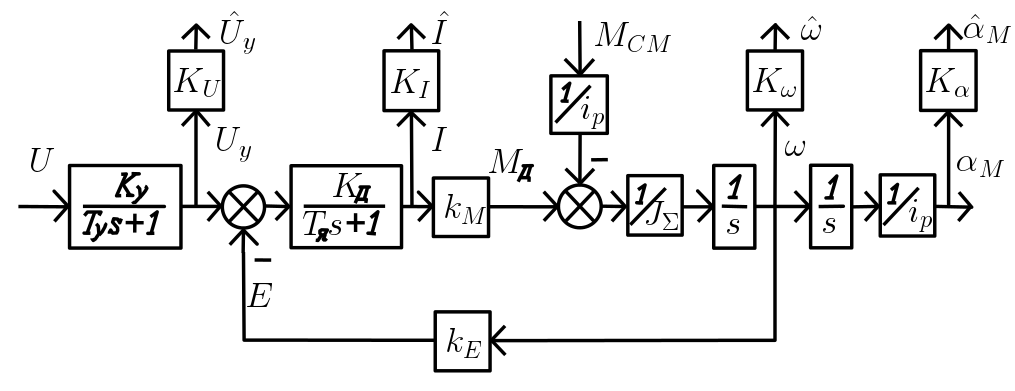
\includegraphics[width = \textwidth]{fullScheme}
		\caption{Структурная схема ЭМО}
		\label{fullScheme}
	\end{figure}
	
	Коэффициенты передачи измерительных устройств $K_U, K_I, K_\omega, K_\alpha$ выбираются таким образом, чтобы обеспечить соответствие максимального значения измеряемого сигнала уровню 10 В на выходе измерительного устройства. Из этого условия имеем:
	\begin{align}
		K_U &= 0,4175\\
		K_I &= 0,419\\
		K_\omega &= 0.19125\\
		K_\alpha &= 12
	\end{align}
	
	Схема модели представлена на рисунке \ref{fullModel}.
	\begin{figure}[ht!]
		\centering
		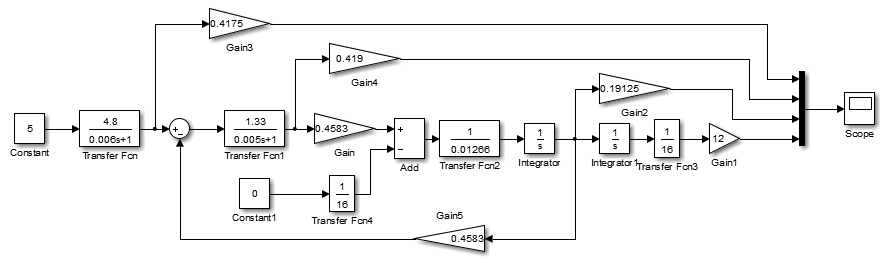
\includegraphics[width = \textwidth]{fullModel}
		\caption{Схема моделирования ЭМО}
		\label{fullModel}
	\end{figure}
	\newpage
	Построим график переходного процесса:
	\begin{figure}[ht!]
		\centering
		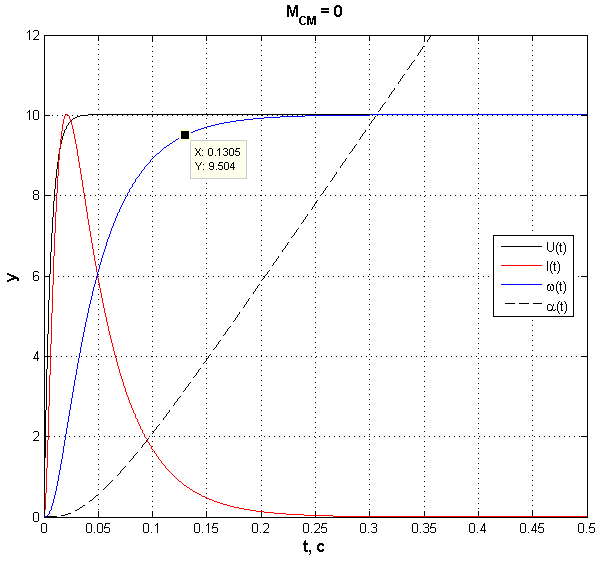
\includegraphics[width = 0.9\textwidth]{M0}
		\caption{График переходного процесса при нулевом моменте сопротивления}
		\label{M0}
	\end{figure}
	\clearpage
	\section{Исследование влияние момента сопротивления на вид переходных процессов}
	\begin{figure}[ht!]
		\centering
		\begin{subfigure}[b]{0.49\textwidth}
			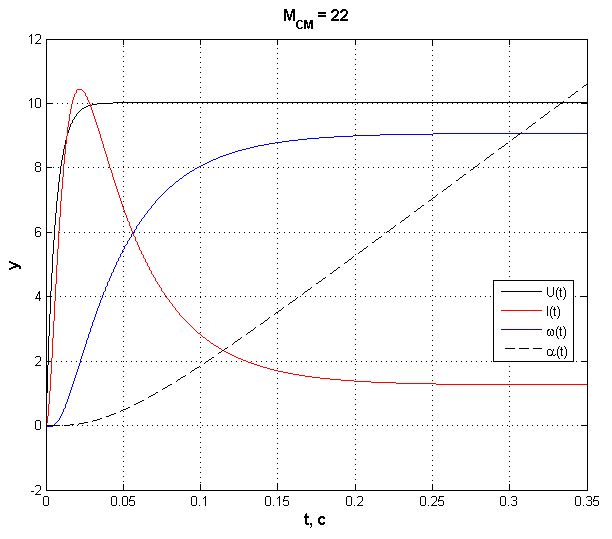
\includegraphics[width = \textwidth]{M22}
		\end{subfigure}
		\hfill
		\begin{subfigure}[b]{0.49\textwidth}
			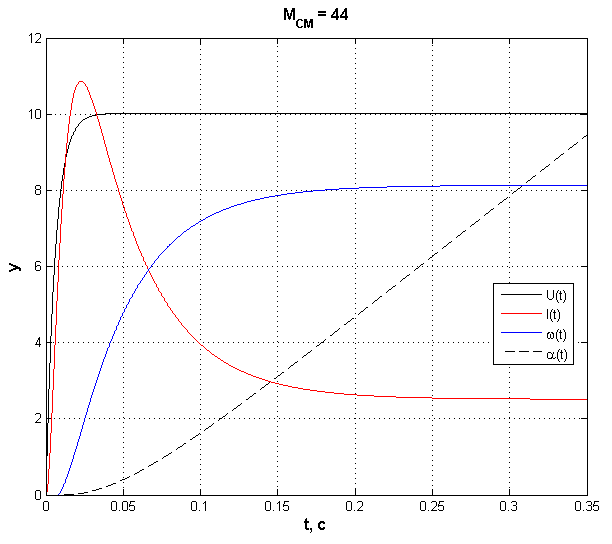
\includegraphics[width = \textwidth]{M44}
		\end{subfigure}
	\end{figure}
	\begin{figure}[ht!]\ContinuedFloat
		\centering
		\begin{subfigure}[b]{0.49\textwidth}
			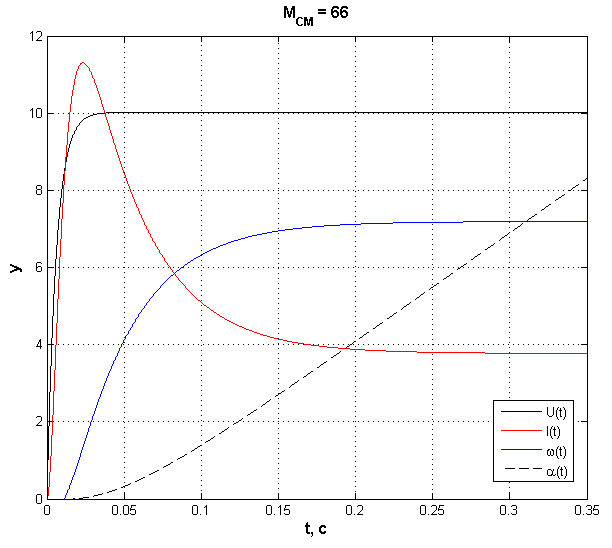
\includegraphics[width = \textwidth]{M66}
		\end{subfigure}
		\hfill
		\begin{subfigure}[b]{0.49\textwidth}
			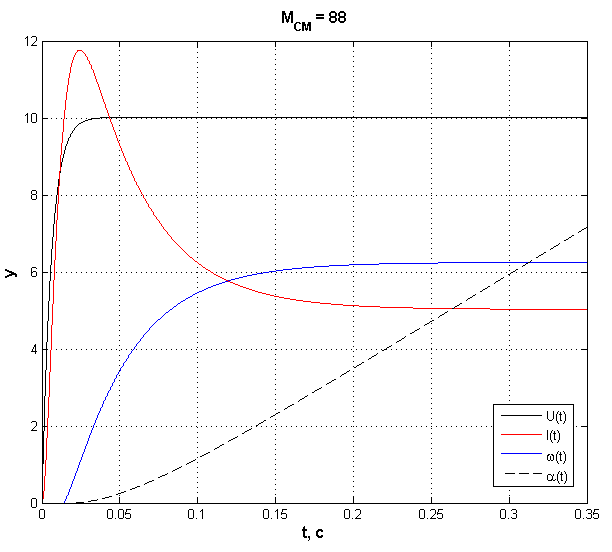
\includegraphics[width = \textwidth]{M88}
		\end{subfigure}
		\caption{Графики переходных процессов при различных значениях момента сопротивления}
		\label{MVar}
	\end{figure}
	Как видно на рисунке \ref{MVar} при увеличении момента сопротивления, время переходного процесса остаётся неизменным и равным 0,13 сек, установившееся значение скорости уменьшается, а тока --- увеличивается.
	\clearpage
	\section{Исследование влияния момента инерции нагрузки на вид переходных процессов}
	\begin{figure}[ht!]
		\centering
		\begin{subfigure}[b]{0.48\textwidth}
			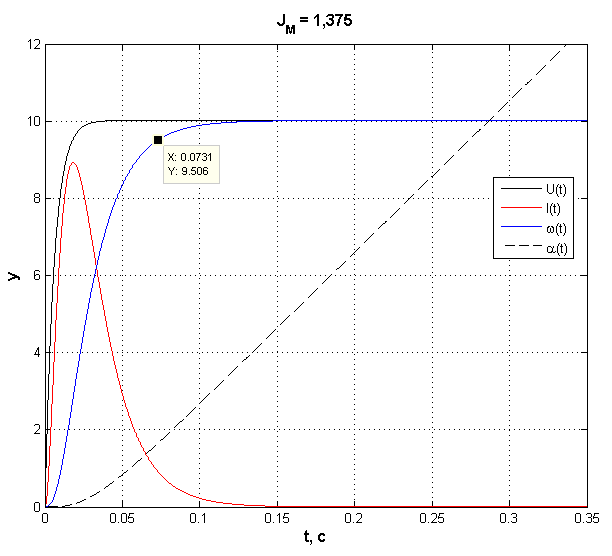
\includegraphics[width = \textwidth]{J1}
		\end{subfigure}
		\hfill
		\begin{subfigure}[b]{0.48\textwidth}
			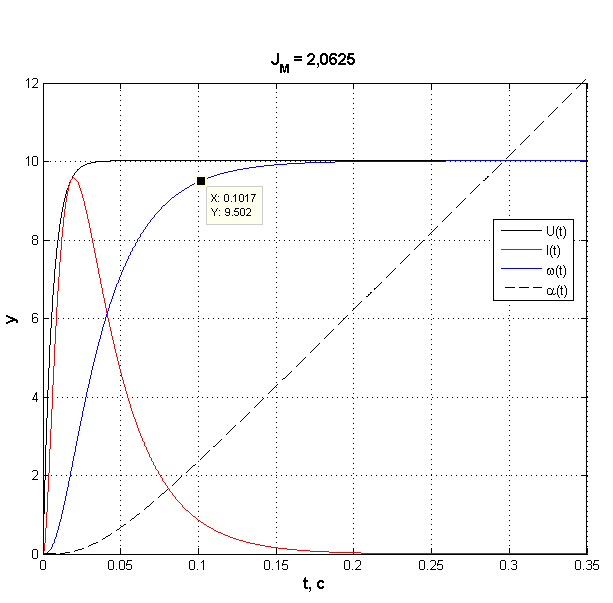
\includegraphics[width = \textwidth]{J2}
		\end{subfigure}
	\end{figure}
	
	\begin{figure}[ht!]\ContinuedFloat
		\centering
		\begin{subfigure}[b]{0.48\textwidth}
			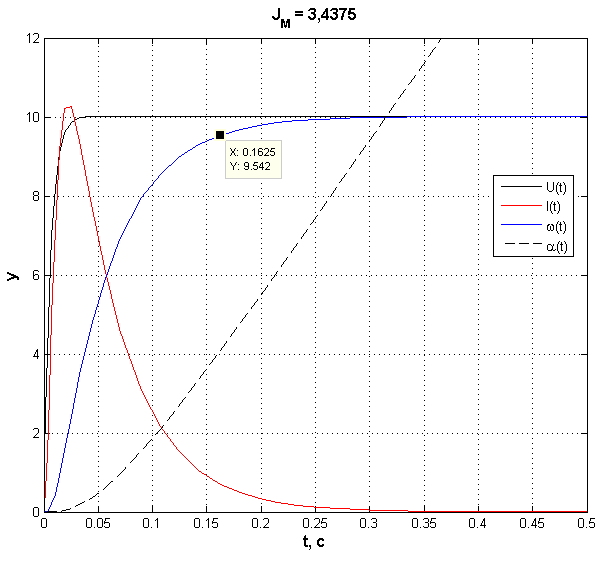
\includegraphics[width = \textwidth]{J3}
		\end{subfigure}
		\hfill
		\begin{subfigure}[b]{0.48\textwidth}
			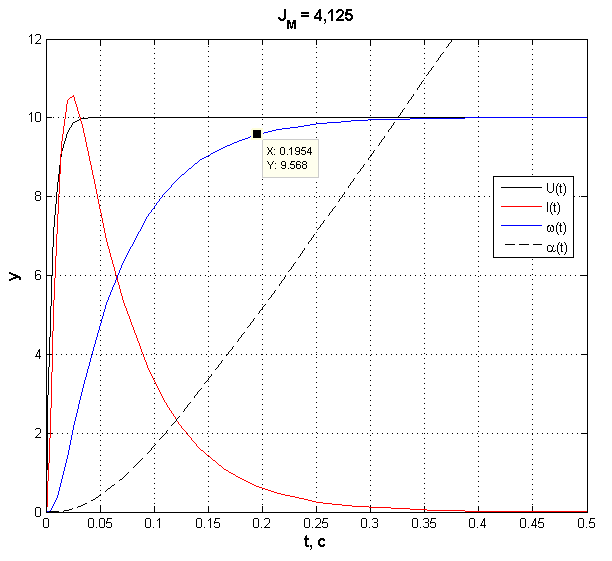
\includegraphics[width = \textwidth]{J4}
		\end{subfigure}
		\caption{Графики переходных процессов при различных значениях момента инерции нагрузки}
		\label{JVar}
	\end{figure}
	Как мы можем наблюдать на графиках переходных процессов, представленных на рисунке \ref{JVar}, время переходного процесса изменяется пропорционально с моментом инерции нагрузки $J_M$, в то время как установившиеся значения тока якоря и угловой скорости остаются неизменными.
	\clearpage
	\section{Исследование влияния передаточного момента редуктора на вид переходных процессов}
	Проведём исследования при величине момента сопротивления $M_{CM} = 0$. Их результаты приведены на рисунке \ref{M0ivar}.
	\begin{figure}[ht!]
		\centering
		\begin{subfigure}[b]{0.49\textwidth}
			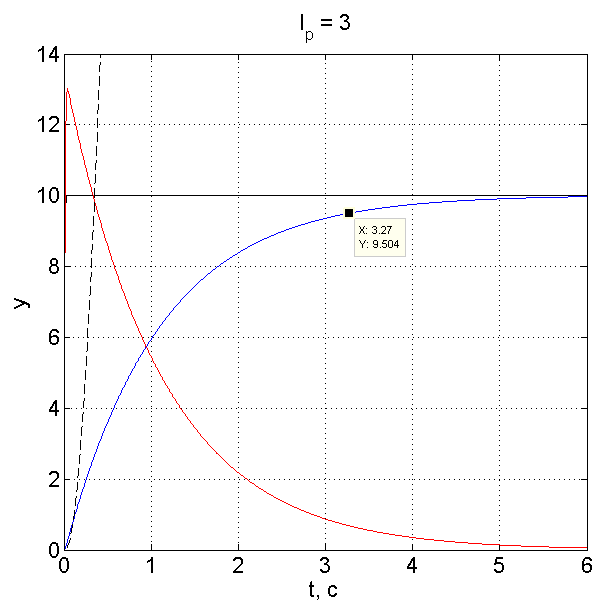
\includegraphics[width = \textwidth]{M0i3}
		\end{subfigure}
		\hfill
		\begin{subfigure}[b]{0.49\textwidth}
			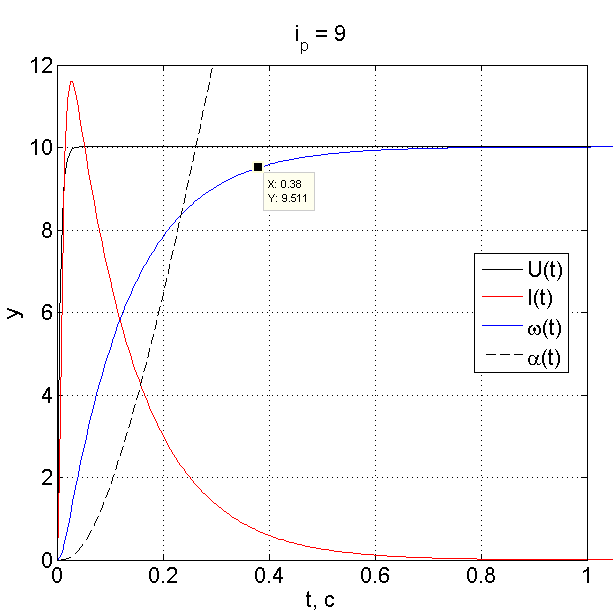
\includegraphics[width = \textwidth]{M0i9}
		\end{subfigure}
	\end{figure}
	\begin{figure}[ht!]\ContinuedFloat
		\centering
		\begin{subfigure}[b]{0.49\textwidth}
			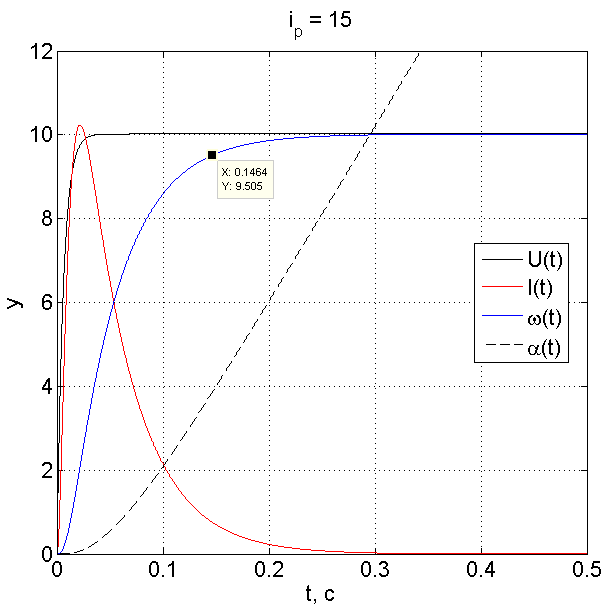
\includegraphics[width = \textwidth]{M0i15}
		\end{subfigure}
		\hfill
		\begin{subfigure}[b]{0.49\textwidth}
			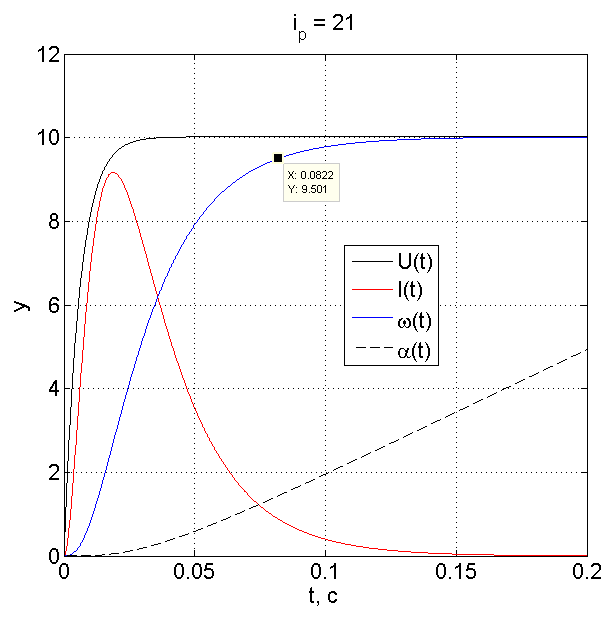
\includegraphics[width = \textwidth]{M0i21}
		\end{subfigure}
		\caption{Графики переходных процессов при нулевом моменте сопротивления и при различных значениях передаточного момента редуктора}
		\label{M0ivar}
	\end{figure}
	
	Как можно заметить по результатам математического моделирования при увеличении передаточного момента редуктора уменьшаются время переходного процесса и максимальное значение тока. Установившиеся значения тока и угловой скорости при этом остаются неизменными.
	
	Так же проведём исследования при величине момента сопротивления $M_{CM} = 44,$ что является равным половине максимального значения, рассчитанного для передаточного момента редуктора $i_p = 16$. Результаты моделирования приведены на рисунке \ref{M44ivar}.
	\begin{figure}[ht!]
		\centering
		\begin{subfigure}[b]{0.45\textwidth}
			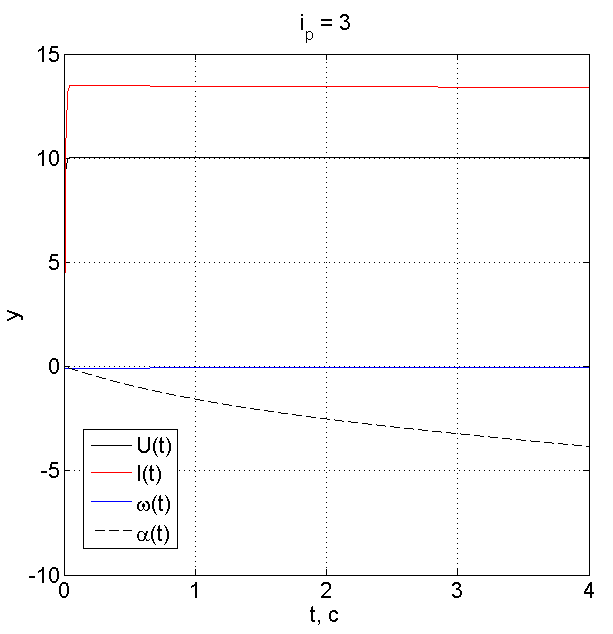
\includegraphics[width = \textwidth]{M44i3}
		\end{subfigure}
		\hfill
		\begin{subfigure}[b]{0.45\textwidth}
			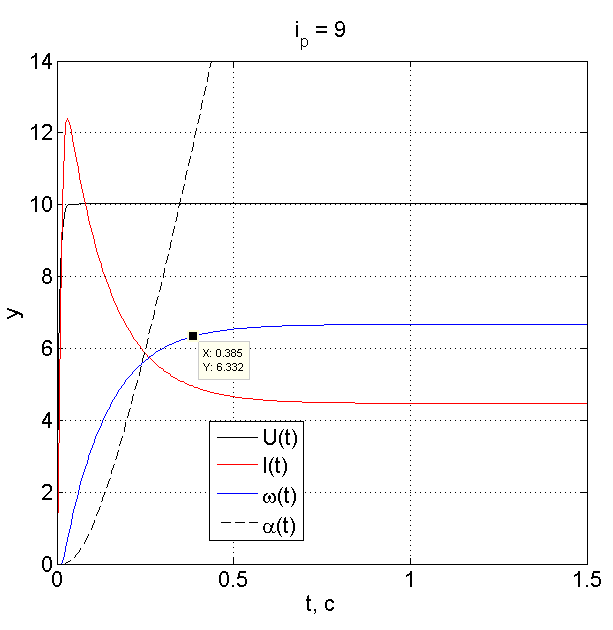
\includegraphics[width = \textwidth]{M44i9}
		\end{subfigure}
	\end{figure}
	\begin{figure}[ht!]\ContinuedFloat
		\centering
		\begin{subfigure}[b]{0.45\textwidth}
			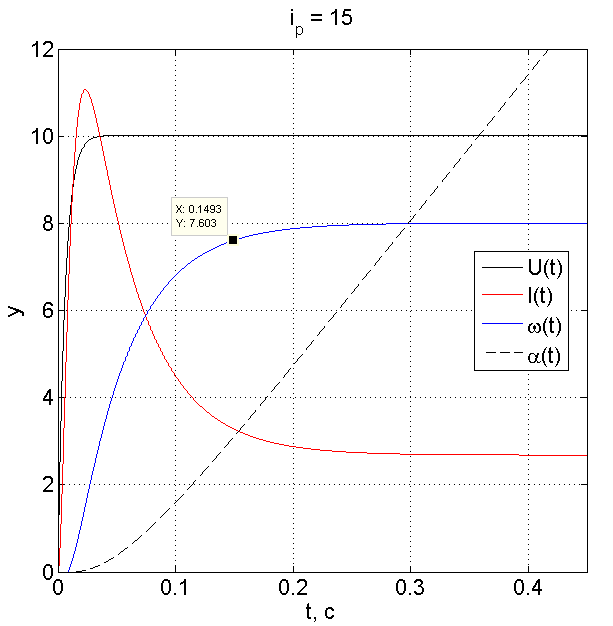
\includegraphics[width = \textwidth]{M44i15}
		\end{subfigure}
		\hfill
		\begin{subfigure}[b]{0.45\textwidth}
			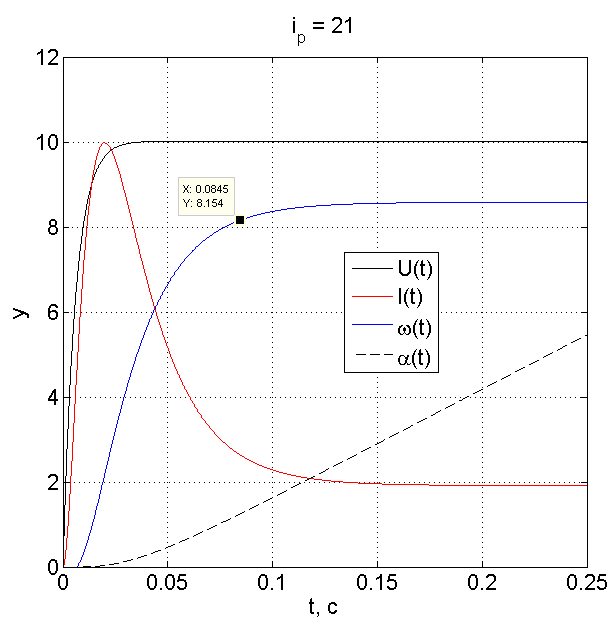
\includegraphics[width = \textwidth]{M44i21}
		\end{subfigure}
		\caption{Графики переходных процессов при ненулевом моменте сопротивления и при различных значениях передаточного момента редуктора}
		\label{M44ivar}
	\end{figure}

	На представленных результатах моделирования видно, что при наличии момента нагрузки и малом показателе передаточного момента редуктора система может не справиться с нагрузкой и никогда не прийти в устойчивое состояние. В нашем случае при значении $i_p = 3$ момента вращения двигателя не хватает, чтобы преодолеть момент сопротивления нагрузки. Так же можно наблюдать, что при увеличении $i_p$ не только уменьшаются значения времени переходного процесса и максимального тока, но и установившиеся значения угловой скорости и тока приближаются к значениям без нагрузки.
	\clearpage
	\section{Исследование влияния значений постоянных времени на вид переходных процессов}
	Для проведения данного исследования уменьшим заданные значения постоянных времени на порядок и получим
	\begin{align}
		T_\text{у} = 0,5 \text{мс} = 0,0005 c\\
		T_\text{я} = 0,6 \text{мс} = 0,0006 c
	\end{align}
	\begin{figure}[ht!]
		\centering
		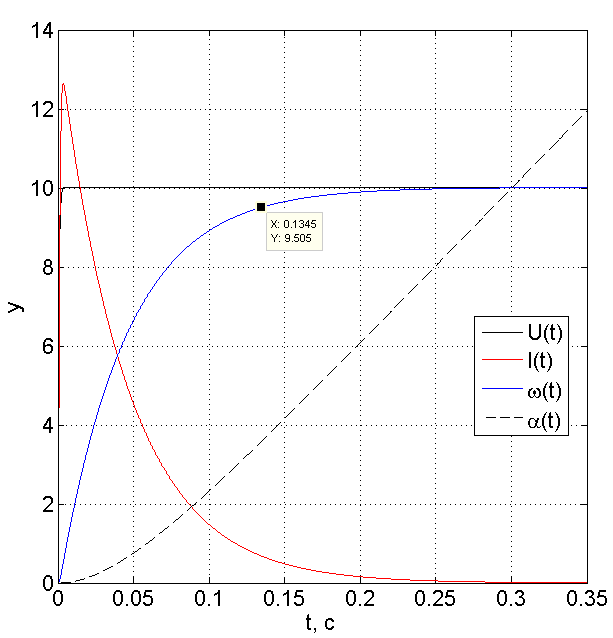
\includegraphics[width = 0.8\textwidth]{Tvar}
		\caption{График переходного процесса при уменьшенных значениях постоянных времени}
		\label{TVar}
	\end{figure}
	
	При уменьшении значений постоянных времени на порядок возросло максимальное значение тока. Время переходного процесса и установившиеся значения тока и скорости остались неизменны.
	\clearpage	
	\section{Математическое моделирование приближённой модели электромеханического объекта}
	Составим упрощённую модель ЭМО на основе структурной схемы, представленной на рисунке \ref{simpScheme}.
	\begin{figure}[ht!]
		\centering
		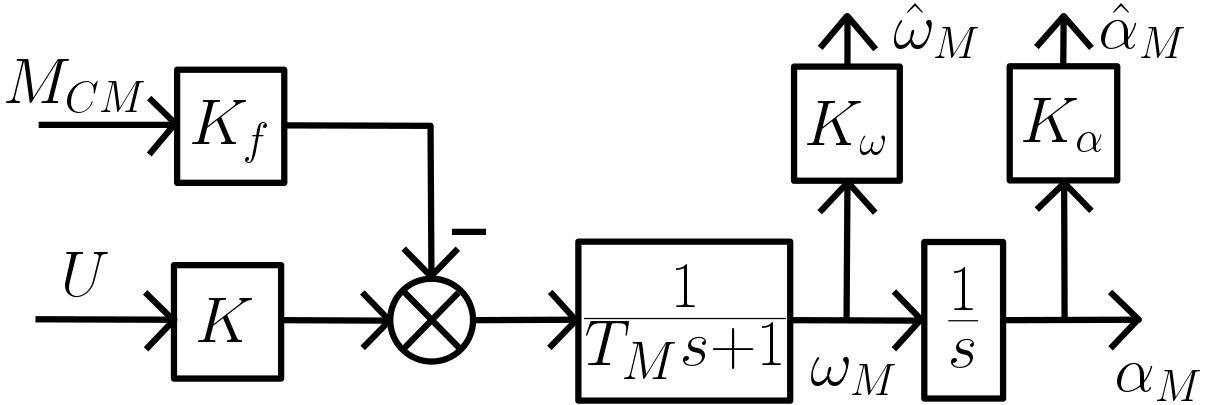
\includegraphics[width = 0.9\textwidth]{simpScheme}
		\caption{Структурная схема упрощённой модели ЭМО}
		\label{simpScheme}
	\end{figure}
	
	Рассчитаем параметры упрощённой ЭМО:
	\begin{align}
		K &= \frac{K_\text{у}}{K_E\cdot i_p} = \frac{4,8}{0,4583 \cdot 16} &= 0,6546\\
		K_f &= \frac{R}{K_M\cdot K_E\cdot i_p^2} = \frac{0,75}{0,4583\cdot0,4583\cdot16^2} &= 0,01395\\
		T_M &= \frac{R\cdot J_\Sigma}{K_M\cdot K_E} = \frac{0,75\cdot0,01266}{0,4583\cdot0,4583} &= 0,0452
	\end{align}
	
	На основе полученных параметров построим математическую модель упрощённой ЭМО. Схема модели приведена на рисунке \ref{simpModel}.
	\begin{figure}[ht!]
		\centering
		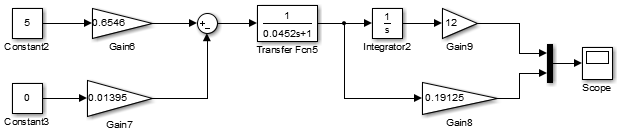
\includegraphics[width = \textwidth]{simpModel}
		\caption{Схема моделирования упрощённой ЭМО}
		\label{simpModel}
	\end{figure}
	\newpage
	Полученный в результате математического моделирования график переходного процесса приведён на рисунке \ref{simpTP}.
	\begin{figure}[ht!]
		\centering
		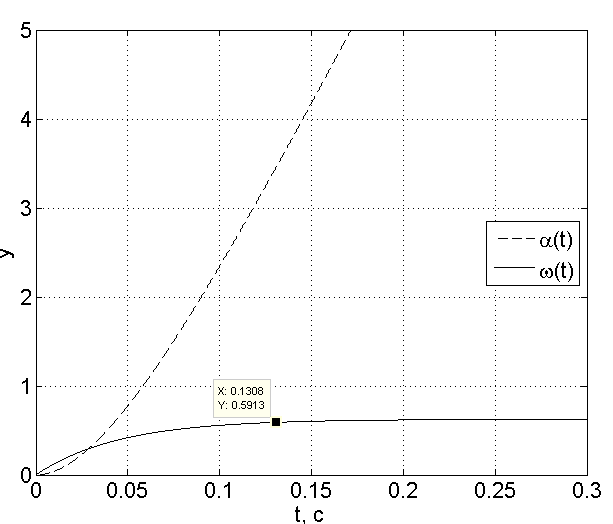
\includegraphics[width = 0.9\textwidth]{simpTP}
		\caption{График переходного процесса упрощённой модели ЭМО}
		\label{simpTP}
	\end{figure}
	
	Исходя из результатов исследования упрощённой модели можно заметить, что значение времени переходного процесса остаётся неизменным, так же как и характер переходного процесса по скорости и углу поворота, но изменяется установившееся значение скорости. Так же на упрощённой модели нет возможности исследования переходных процессов для тока и напряжения.
	\clearpage
	\section*{Вывод}
	В ходе работы было показано, как различные параметры, такие как момент сопротивления нагрузки, передаточный момент редуктора и постоянные времени влияют на показатели переходных процессов системы и её работоспособность в целом.
	
	Так же была исследована упрощённая модель электромеханического объекта и в ходе математического моделирования было показано, что её можно использовать для определения времени и характера переходного процесса по скорости.
\end{document}